% !TEX root = paper/paper.tex
\title{Prediction with Features Missing at Test Time}

\author{
Sergey Karayev \\
UC Berkeley
}

\nipsfinalcopy
\begin{document}
\maketitle

\begin{abstract}
We look at prediction with all features available at training time, but only a subset observed at test time.
Such situations may arise due to sensor loss, or when using test-time instance-specific feature selection.
We examine three areas of modeling choices:

\begin{enumerate}
\item For imputation, we look at mean, SVD, joint Gaussian conditioning, and nearest neighbor methods.

\item For classification, we evaluate augmenting the training data with imputed values, modifying the loss function to consider the expected feature ``corruption'', and using non-linear classifiers.

\item We additionally evaluate training different classifiers for different subsets of observed features.
\end{enumerate}

We evaluate reconstruction and classification error on two datasets: Digits and Scenes-15.
Two feature selection policies are considered: Random and Clustered.
For each policy, we consider Independent and Block-wise selection patterns.

We find that mean imputation with classifier retraining is a reasonably well-performing approach.
Nearest Neighbor methods perform best but are the most expensive.
Gaussian imputation method performs very well, but is also expensive.

Training classifiers with a loss function modified to expect a certain level of feature corruption did not improve performance.
Training additional classifiers for clusters of observed feature subsets did not improve performance.

\end{abstract}

\section{Introduction}
In supervised prediction problems, \emph{features} extracted from inputs are combined to output a real value (regression) or a label (classification).
The goal of training is to minimize the \emph{loss} of the predictions with the true values or labels---for example, the accuracy of classification.

We look at a complication of this problem.
While all features are available at training time, only a subset of features of each instance is observed at test time.
Such situations can arise in real world deployments of predictive systems due to sensor failure.
Another motivation for the problem comes from work on dynamic feature selection: to predict with minimum loss on a fixed time budget, different subsets of features are extracted for different instances \cite{Karayev-NIPS-2012, Xu-ICML-2013}.

Since the training set is fully observed, we can train a classifier with all features.
At test time, we could attempt to impute the unobserved feature values given the observed ones, and use the classifier trained on the fully observed training set.
There are many methods of imputing missing values, differing in their power and cost.
We consider: simple mean imputation; singular value decomposition-based imputation; multivariate Gaussian conditioning; and nearest neighbor imputation with two similarity measures.

In addition to imputing at test time, we can apply the test-time observation process to the training data, impute values, and re-train the classifier.
This amounts to a regularization that prevents the classifier from relying on any single feature, as it may not be in the observed subset.
Taking this idea further, we could work the expected feature ``corruption'' into the loss function of the linear classifier, which is equivalent to augmenting the training set with an infinite amount of corrupted data.

The feature selection process may not select features independently.
It could select features by block instead of one by one, and it could have a bound on the total number of unique subsets that are selected.
We evaluate in these conditions, and notice that if there is a small bound on the number of subsets, then we can learn a separate classifier for each subset of observed features.
Even if the bound is not small, we may still derive benefit from training more than one classifier, and at test time using the classifier trained on the closest subset of features to the observed instance.

\subsection{Related Work}
The imputation problem is faced in the \emph{collaborative filtering} literature, working on problems such as the Netflix Prize \cite{Koren-2009}.
Matrix factorization methods, commonly based on the Singular Value Decomposition (SVD), are often employed.
Our SVD imputation method is inspired by this literature.
However, the training data is also missing values in this problem, and the end goal is not classification with imputed features, which makes it different from ours.
Imputation approaches have also been explored in genomics work, where the real-world data is often missing a large portion of the observations \cite{Hastie-1999}.

Our main motivating case is the problem of test-time dynamic feature selection.

Locally-weighted regression, corresponding to a mixture of Gaussians model, was used for the classification task in \cite{Gao-NIPS-2011}.
A discrete Markov Random Field model, with Belief Propagation inference, was used in \cite{Karayev-NIPS-2012}.
Both of the approaches are computationally expensive; the first scales very poorly with both dataset size and feature dimensions, the second with number of classes.

If the number of possible observed subsets is bounded, then a separate classifier can be learned for each subset---this is done in the tree-structured dynamic policy of \cite{Xu-ICML-2013}.
We do not want to be limited to a tree structure, and so would like a more general method.

An interesting related problem is explored in work on feature corruption, for example the ``Nightmare at test time'' scenario of \cite{Globerson-ICML-2006}, and the Marginalized Corrupted Features of \cite{Maaten-ICML-2013}.
These approaches modify the loss function of a linear classifier with, respectively, the worst-case or the expected-case of feature corruption.
Because they provide additional regularization of the classifier weights, such approaches may increase performance even if there is no test-time corruption.
On our task, however, they are outperformed by simpler baselines.

\section{Problem Formulation}


\begin{mydef} \label{def:problem}
\textbf{The prediction problem} consists of
\begin{itemize}
\item Set $\mathcal{D}$ of $N$ instances of $K$ possible labels: $\mathcal{D} = \{x_n \in \mathcal{X}, y_n \in \{1, \dots, K\}\}_{n=1}^N$.

\item Set $\mathcal{H}$ of $F$ features $\mathcal{H} = \{h_f : \mathcal{X} \mapsto \mathbb{R} \}_{f=1}^F$.\\
To represent featurized instance, we write $\mathbf{x} = [h_0(x), h_1(x), \dots, h_f(x)]$.

\item Test-time feature selection function $o(x, b): \mathcal{X} \times \mathbb{R} \mapsto \mathbb{B}^F$, where $\mathbb{B} \in \{0, 1\}$, and $b \in [0, 1]$ is given and specifies the fractional selection \emph{budget}.

\item Loss function $\ell(g(x), y): \mathbb{R}^K \times \{1, \dots, K\} \mapsto \mathbb{R}$.
\end{itemize}

Given $b$, we seek a procedure $g(x)$ that minimizes total loss $\sum \ell(g(x_n), y_n)$ under the condition that $o(x, b)$ is applied to each $x$.
\end{mydef}

Applied to $x$, $o(x, b)$ gives the binary selection vector $\mathbf{o}$ which splits $\mathbf{x}$ it into observed and unobserved parts such that $\mathbf{x}^m = [\mathbf{x}^\text{o}, \mathbf{x}^\text{u}]$.

$X^c$ denotes the fully observed $N \times F$ training set.
We assume that we have only sequential access to the missing-feature test instances $\mathbf{x}^m$.

We see three experimental conditions: (1) how to fill in missing values; (2) which loss function to use in learning the classifier and whether to augment the training data; (3) how many classifiers to learn.

\section{Imputing missing values}
Our training data is complete, allowing us to train classifiers that use all features.
It is reasonable to fill in---\emph{impute}---the missing values of test data, such that we can use the trained classifiers without modification.

\subsection{Mean}
We simply replace the missing value in $X^m$ with their row mean in $X^c$.
Because our data is always zero-mean, this amounts to simply replacing the value with $0$.

\subsection{SVD Imputation}
The basic idea is to learn a set of basis function using the Singular Value Decomposition (SVD) of the matrix $X^c$, and impute missing values in $X^m$ by regressing to the basis functions using the observed values, and using the regression coefficients to predict the missing values.

The rank-$R$ truncated SVD of $N \times F$ matrix $X^c$ can be written as
\begin{equation}
\hat{X}^c = U_R D_R V_R^T
\end{equation}
where $U$ is an $N \times R$ matrix of left singular vectors, $V$ is an $F \times R$ matrix of right singular vectors, and $D$ is a diagonal matrix of the top $R$ singular values of $X^c$.

It can be proven \cite{Hopcroft-book-2013} that $U$ and $V$ are orthogonal, and that the truncated SVD is the best rank-$R$ approximation to $X^c$:
\begin{equation}
\min_{M\,\text{of rank}\,J} || X^c - M ||_F
\end{equation}

To set up the imputation, let's view this result from the angle of least-squares regression of a row $x$ of $X^c$ onto the right singular vectors:
\begin{equation} \label{eq:svd_regression}
\min_\theta \sum_{f=1}^F (x_f - \sum_{r=1}^R v_{fr} \theta_r )^2 = \min_\theta \left\| x - V_R \theta \right\|
\end{equation}

The solution is given in closed form by $\left( V_R^T V_R \right)^{-1} V_R^T x$, and as $V_R$ is orthogonal, we obtain $\theta = V_R^T x$.
A row is predicted as $\hat{x} = V_R \theta$, and the whole matrix as $\hat{X^c} = \Theta V_R^T$.
$\Theta = X^c V_R = U_R D_R$ gives regression coefficients for all rows, and so $\hat{X}^c = U_R D_R V_R^T$.

We see that the SVD performs regression of $X^c$ onto $V_R$.
Now consider the missing-value matrix $X^m$.
The same regression can be performed, using only observed values:
\begin{equation}
\min_\theta \sum_{f \text{obs}} (x_f - \sum_{r=1}^R v_{fr} \theta_r )^2 = \min_\theta \left\| x - V_R^\text{o} \theta \right\|
\end{equation}
where $V_R^o$ is a version of $V_R$ composed only of rows corresponding to observed features in $x$.

The solution is now given by $\theta = \left( V_R^{\text{o}T} V_R^o \right)^{-1} V_R^{\text{o}T} x$ ($V^\text{o}$ is not necessarily orthogonal), and the predictions for the missing elements of $x$ are $V_R^\text{u} \theta$, where $V_R^\text{u}$ is the complement to $V_R^\text{o}$, composed only of rows corresponding to unobserved features in $x$.

Note that we do not need an intercept term for these regressions, as each column of $X$ is zero-mean.

\paragraph{Parameters}
$R$ is a parameter of this approach.
As $N > F$ in all of our evaluation, the largest value that $R$ can take on is $F$.
Using a smaller value may in fact be beneficial as it may rid the data of noise, but there is no theory to guide us.

We set $R$ via 3-fold cross-validation on the training set.

\paragraph{Computational Complexity}
There are numerous algorithms for computing the SVD, but the runtime is usually dominated by a $O(N^3)$ operation, which scales poorly with the size of the dataset.
Computing the full SVD is also very memory-intensive---prohibitively so for even medium-sized datasets (on the order of 1000x1000).
Computing the truncated SVD, which is all we need, can be done with constant memory, but remains slow in all implementations considered.

\subsection{Joint Gaussian model}

We can make a modeling assumption that allows another imputation method.
Specifically, we assume that $\mathbf{x}$ is distributed according to a multivariate Gaussian $\mathbf{x} \sim \mathcal{N}(\mathbf{0}, \Sigma)$, where $\Sigma$ is the sample covariance $X^T X$ and the data is standardized to have zero mean.

For a test instance with missing features, we can write
\begin{equation}
\mathbf{x} = \begin{bmatrix} \mathbf{x}^\text{o}\\  \mathbf{x}^\text{u} \end{bmatrix} \sim \mathcal{N} \left( \mathbf{0}, \begin{bmatrix} \mathbf{A} & \mathbf{C}\\ \mathbf{C}^T & \mathbf{B} \end{bmatrix} \right)
\end{equation}
where $\mathbf{A}$ is the covariance matrix of $\mathbf{x}^\text{o}$, $\mathbf{B}$ is the covariance matrix of $\mathbf{x}^\text{u}$, and $C$ is the cross-variance matrix that has as many rows as the size of $\mathbf{x}^\text{o}$ and as many columns as the size of $\mathbf{x}^\text{u}$ \cite{Roweis-gaussian-identities}.

In this case, the distribution over unobserved variables conditioned on the observed variables is given by
\begin{equation}
\mathbf{x}^\text{u} \mid \mathbf{x}^\text{o} \sim \mathcal{N} \left( \mathbf{C}^T \mathbf{A}^{-1} \mathbf{x}^\text{o},\, \mathbf{B} - \mathbf{C}^T \mathbf{A}^{-1} \mathbf{C} \right)
\end{equation}

\paragraph{Parameters}
In this approach, we can choose to either always set the imputed values to the mean of the conditional Gaussian, or to impute with noise specified by the covariance matrix.
In preliminary experiments, using the mean only provided far better performance, so only that setting is included in the evaluation.

\paragraph{Computational Complexity}
After computing the complete covariance matrix $\Sigma$, which takes $O(N^3)$ time, we need to make $N'$ test-time predictions.
In the course of the predictions, we may need to compute at most $\min(N', 2^F)$ unique matrix inversions (again in $O(N^3)$).
The size of the matrices being inverted is proportional to the budget $b$, making this method slower for larger budgets.

\subsection{k-NN Imputation and Prediction}
In the SVD and Gaussian methods, we want to use some knowledge of the feature covariance to fill in the missing values.
Instead of learning anything, we could go directly to the source of the covariances---the actual feature values for all points in the training set.
The family of Nearest Neighbor methods takes this approach.
The algorithm for imputation is simple: find the nearest neighbors in the observed dimensions, and use their averaged values to fill in the unobserved dimensions.

For $\mathbf{X}^m$, we find the $k$ nearest neighbors with the highest dot product similarity $\mathbf{x}^{cT} \mathbf{x^m}$ or lowest Euclidean distance $\| \mathbf{x}^{c} - \mathbf{x}^{m} \|$, using only the features that are observed in $\mathbf{x}^{m}$.

For \textbf{imputation}, the unobserved values are set to the average across these nearest neighbors for that dimension.
Similarly, we do \textbf{classification} by returning the mode label of the nearest neighbors.

\paragraph{Parameters}
The obvious parameter of $k$-NN is $k$, which we set by 3-fold cross-validation on the training set (up to $20$).

\paragraph{Computational Complexity}
Finding the nearest neighbors by dot product similarity is $O(NF'^2)$, and Euclidean distance is the same with an additional constant term.
$F'S$ is the number of observed dimensions, which grows proportionally with budget $b$, making this method more expensive with increased budget.

\section{Classifiers}

In addition to the $k$-NN classifier described above, we consider three linear classifiers, obtained by minimizing:
\begin{enumerate}
  \item Logistic loss on fully observed data: simply using $X^c$.
  \item Logistic loss on synthetically re-imputed version of the data: we obtain $X^m$ through applying $o(x, b)$ on each $x^c$, and then imputing the missing values with the methods described.
  \item Logistic and quadratic loss derived with Marginalized Corrupted Features (MCF) \cite{Maaten-ICML-2013}.
\end{enumerate}

The idea of (3) is to move the expectation of feature corruption into the loss function, which is equivalent to adding an infinite amount of corrupted data to the training set.
Remarkably, this is not any more computationally complex than the standard loss (although minimization does take longer, empirically).

For example, for blankout noise and logistic loss, we can derive the surrogate loss
\begin{equation}
\mathcal{L}(D; \mathbf{\theta}) \leq \sum_{n=1}^N \log \left( 1 + \prod_{f=1}^F \left[ q_f + (1 - q_f) e^{-y_n \theta_f \frac{1}{1 - q_d} x_{nf}} \right] \right)
\end{equation}

For additional loss functions, see \cite{Maaten-ICML-2013}.

\subsection{Clustering classifiers}

The binary selection vectors $\mathbf{o}$ may not be generated independently.
In particular, there may only be a few unique selection vectors that are applied to all test-time instances.
If the number of the unique masks is small, then a separate classifier can be learned for each one, using the full training set, appropriately masked.

Extending the idea, even in the case of a large number of unique masks, we can learn several classifiers instead of just one.
In the case of training $K$ classifiers, we need to find $K$ clusters such that the masks are distributed as evenly as possible into the clusters.
We use hierarchical agglomerative clustering for this task, growing clusters bottom-up from the observed masks obtained by running $o(x, b)$ on the training instances $x^c$.
The distance measure for the binary masks is the Hamming distance; standard K-Means clustering technique is not applicable to this distance measure.

\section{Evaluation}

Feature selection had four experimental conditions.

\begin{itemize}
\item
In \textbf{Random, Independent} selection, each feature was selected independently, and the total number of possible masks for a given budget was not bounded, such that each test instance could have a unique mask (if the number of test instances $N$ was less than the total number of possible feature subsets $2^F$.

\item
In \textbf{Random, Block-wise} selection, there was no bound on the number of possible masks for a given budget, but features were selected by blocks.

\item
In \textbf{Clustered, Independent} selection, each feature was selected independently, but there were at most $K$ possible masks for a given budget.

\item
In \textbf{Clustered, Block-wise} selection, there were at most $K$ possible masks for a budget, and features were selected by blocks.
\end{itemize}

The MCF method is only evaluated in the \textbf{Random, Independent} policy setting, most advantageous to its assumptions.

All datasets were first standardized by subtracting the row mean and dividing by the row standard deviation.

\subsection{Digits}
The Digits dataset contains 8x8 grayscale images of hand-written digits 1-10.
Each of the 10 classes has 200 samples, for a total of 2000 images and 64 features.

The dataset was split 60-40 into training and testing sets.
The number of clusters for clustered selection was 10.
For block-wise feature selection, the number of blocks was set to 8.

Figure~\ref{fig:digits} shows the results; here we summarize the conclusions:
\begin{itemize}
\item Mean imputation has highest reconstruction and classification error, aside from SVD, which was so bad that its curves were not plotted.
\item Dot product-based kNN imputation performs worse than Gaussian imputation for both reconstruction and classification, and is slower.
\item Euclidean distance-based kNN imputation performs best, but is slowest.
\item Retraining classifier with mean imputation makes a big difference, while retraining classifier with Gaussian imputation does not make a difference at all.
Presumably, Gaussian imputation maintains the feature statistics of the fully-observed classifier sufficiently well.
\item Modifying the loss function with MCF results in worse performance than doing mean imputation and retraining (MCF evaluated only on the \textbf{Random, Independent} policy).
\item Training additional classifiers for clusters of observed susbets does not make a difference to classification performance.
\item These results hold for all policy experimental conditions.
\end{itemize}

\begin{figure}[ht!]
    \centering
    \begin{subfigure}[b]{\textwidth}
        \centering
        \includegraphics[width=.9\textwidth]{../../figures/281b/digits/random_-1/subplots.png}
        \caption{Random, independent feature selection.\vspace{.2cm}}
    \end{subfigure}
    \begin{subfigure}[b]{\textwidth}
        \centering
        \includegraphics[width=.9\textwidth]{../../figures/281b/digits/random_8/subplots.png}
        \caption{Random, block-wise (8 blocks) feature selection.\vspace{.2cm}}
    \end{subfigure}
    \begin{subfigure}[b]{\textwidth}
        \centering
        \includegraphics[width=1\textwidth]{../../figures/281b/digits/clustered_-1/subplots.png}
        \caption{Clustered (10 clusters), independent feature selection.\vspace{.2cm}}
    \end{subfigure}
    \begin{subfigure}[b]{\textwidth}
        \centering
        \includegraphics[width=1\textwidth]{../../figures/281b/digits/clustered_8/subplots.png}
        \caption{Clustered (10 clusters), block-wise (8 blocks) feature selection.\vspace{.2cm}}
    \end{subfigure}

    \small{
    \begin{subfigure}[b]{1\textwidth}
        \centering
        \begin{tabular}{ll}
\toprule
                                   & clustered\\
\midrule
gaussian, full                     & 0.206\\
gaussian, retrained                & 0.206\\
kNN (dot)                          & 0.241\\
kNN (dot), full                    & 0.211\\
kNN (euclidean)                    & \textbf{0.166}\\
kNN (euclidean), full              & 0.170\\
mean, full                         & 0.308\\
mean, retrained                    & 0.223\\
mean, retrained, 5 clusters        & 0.301\\
mean, retrained, all (10) clusters & 0.194\\
\bottomrule
\end{tabular}

        \caption{Areas under the Classification Error vs. Budget curves. Lower is better.}
    \end{subfigure}
    \begin{subfigure}[b]{1\textwidth}
        \centering
        \begin{tabular}{lllll}
\toprule
                & clustered & clustered, blocks & clustered & clustered, blocks\\
\midrule
gaussian        & 94.76     & 93.16             & 151.43    & 150.06\\
kNN (dot)       & 102.5     & 97.59             & 180.11    & 170.79\\
kNN (euclidean) & 87.33     & 87.16             & 159.33    & 159.09\\
mean            & 120.08    & 114.02            & 252.38    & 237.75\\
\bottomrule
\end{tabular}


        \caption{Areas under the Reconstruction RMSE vs. Budget curves. Lower is better.}
    \end{subfigure}
    }
    \caption{All results on the \textbf{Digits} dataset.}
    \label{fig:digits}
\end{figure}

\subsection{Scenes-15}
The Scene-15 dataset \cite{Lazebnik-CVPR-2006} contains 4485 images from 15 visual scene classes.
The task is to identify classify images according to scene.

Following \cite{Xiao-CVPR-2010}, we extracted 14 different visual features (GIST, HOG, TinyImages, LBP, SIFT, Line Histograms, Self-Similarity, Textons, Color Histograms, and variations).
Separate multi-class linear SVMs were trained on each feature channel, using a random 100 positive example images per class for training.
We used the liblinear implementation, and cross-validated the penalty parameter $C$.

The trained SVMs were evaluated on the images not used for training, resulting in a dataset of 2238 vectors of 210 confidence values: 15 classes for each of the 14 feature channels.
This dataset was split 60-40 into training and test sets for our experiments.
The number of clusters for clustered selection was 10.
For block-wise feature selection, the number of blocks was set to 5.

Figure~\ref{fig:scenes} shows the results.
The conclusions are much the same as for the \textbf{Digits} dataset, with the following additional observations:
\begin{itemize}
\item Gaussian imputation is more costly than kNN on this data; the feature dimensions is more than twice that of the Digits data.
\item For block-wise feature selection, mean imputation with retraining is as good as any other approach, and of course by far the fastest.
\end{itemize}

\begin{figure}[ht!]
    \centering
    \begin{subfigure}[b]{\textwidth}
        \centering
        \includegraphics[width=.9\textwidth]{../../figures/281b/scenes/random_-1/subplots.png}
        \caption{Random, independent feature selection.\vspace{.2cm}}
    \end{subfigure}
    \begin{subfigure}[b]{\textwidth}
        \centering
        \includegraphics[width=.9\textwidth]{../../figures/281b/scenes/random_5/subplots.png}
        \caption{Random, block-wise (8 blocks) feature selection.\vspace{.2cm}}
    \end{subfigure}
    \begin{subfigure}[b]{\textwidth}
        \centering
        \includegraphics[width=1\textwidth]{../../figures/281b/scenes/clustered_-1/subplots.png}
        \caption{Clustered (10 clusters), independent feature selection.\vspace{.2cm}}
    \end{subfigure}
    \begin{subfigure}[b]{\textwidth}
        \centering
        \includegraphics[width=1\textwidth]{../../figures/281b/scenes/clustered_5/subplots.png}
        \caption{Clustered (10 clusters), block-wise (8 blocks) feature selection.\vspace{.2cm}}
    \end{subfigure}

    \small{
    \begin{subfigure}[b]{1\textwidth}
        \centering
        \begin{tabular}{ll}
\toprule
                                   & clustered\\
\midrule
gaussian, full                     & 0.206\\
gaussian, retrained                & 0.206\\
kNN (dot)                          & 0.241\\
kNN (dot), full                    & 0.211\\
kNN (euclidean)                    & \textbf{0.166}\\
kNN (euclidean), full              & 0.170\\
mean, full                         & 0.308\\
mean, retrained                    & 0.223\\
mean, retrained, 5 clusters        & 0.301\\
mean, retrained, all (10) clusters & 0.194\\
\bottomrule
\end{tabular}

        \caption{Areas under the Classification Error vs. Budget curves. Lower is better.}
    \end{subfigure}
    \begin{subfigure}[b]{1\textwidth}
        \centering
        \begin{tabular}{lllll}
\toprule
                & clustered & clustered, blocks & clustered & clustered, blocks\\
\midrule
gaussian        & 94.76     & 93.16             & 151.43    & 150.06\\
kNN (dot)       & 102.5     & 97.59             & 180.11    & 170.79\\
kNN (euclidean) & 87.33     & 87.16             & 159.33    & 159.09\\
mean            & 120.08    & 114.02            & 252.38    & 237.75\\
\bottomrule
\end{tabular}


        \caption{Areas under the Reconstruction RMSE vs. Budget curves. Lower is better.}
    \end{subfigure}
    }
    \caption{All results on the \textbf{Scenes-15} dataset.}
    \label{fig:scenes}
\end{figure}

\section{Conclusion}

On both datasets, and for all feature selection approaches, we find that mean imputation (with a classifier trained on imputed data) is a well-performing approach.
Nearest Neighbor and Gaussian methods perform best but are the most expensive; Gaussian scales poorly with number of features, while NN scales poorly with size of training set.

We did not find that using Marginalized Corrupted Features loss function improved classification performance.
In fact, the simple baseline approach of mean imputation with classifier retraining performed better.
Training additional classifiers for clusters of observed feature subsets also did not improve performance on these datasets.
Further study of this method is needed.
